% !TEX program = pdflatex
\documentclass{article}
\usepackage{tikz}
\usetikzlibrary{patterns}

\begin{document}
\section*{A section through the filter}
\begin{figure}[ht]\centering
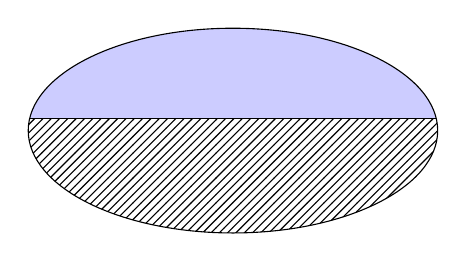
\begin{tikzpicture}

\begin{scope}\clip (0,0) ellipse (2.6 and 1.3);
\fill[pattern=north east lines] (-3,-2) rectangle (3,.15);
\fill[blue!20] (-3,.15) rectangle (3,2);
\draw (-3,.15)--(3,.15);\end{scope}
\draw (0,0) ellipse (2.6 and 1.3);
\end{tikzpicture}\caption{Hatching marks the granular bed below the water.}\end{figure}
\end{document}
